\documentclass[12pt, a4paper]{article}

\usepackage{amsmath}
\usepackage{amssymb}
\usepackage{geometry}
\usepackage{tikz}
\usepackage{hyperref}
\usepackage{parskip}
\usepackage{titlesec}
\usepackage{xcolor}

\geometry{margin=2.5cm}

\hypersetup{
    colorlinks=true,
    linkcolor=black,
    urlcolor=blue
}

\title{\textbf{Maximum Number of Segments Connecting \\ the Vertices of a Polygon}}
\author{}
\date{}

\begin{document}

\maketitle

\section*{Problem Statement}

Given a convex polygon with $n$ vertices, how many distinct line segments can be drawn by connecting every pair of vertices?

\section*{Setup}

A polygon with $n$ sides has exactly $n$ vertices, and initially contributes $n$ segments, namely its \emph{sides}. In addition to the sides, we must also count the \emph{diagonals} — the segments that connect two non-adjacent vertices, passing through the interior of the polygon.

\section*{Illustrative Examples}

The figures below show the complete set of segments for polygons with 3, 4, and 5 vertices, respectively.

\begin{center}
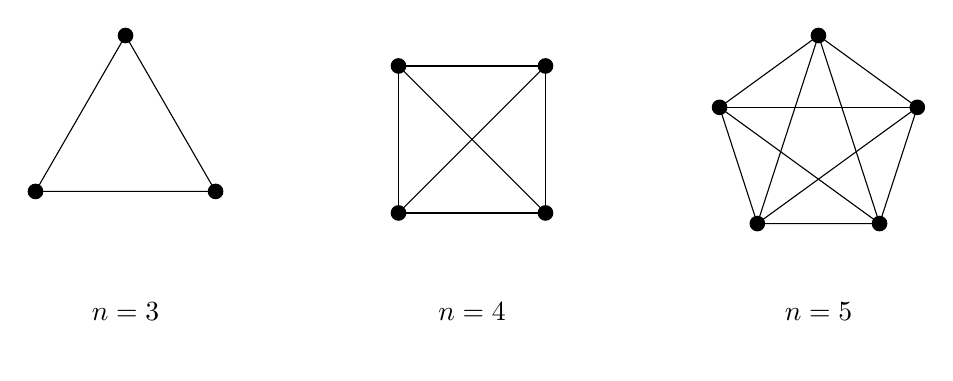
\begin{tikzpicture}[scale=1.1, every node/.style={circle, fill=black, inner sep=2pt}]

% Triangle (n=3)
\begin{scope}[xshift=0cm]
  \coordinate (A) at (90:1.2);
  \coordinate (B) at (210:1.2);
  \coordinate (C) at (330:1.2);
  \draw (A) -- (B) -- (C) -- cycle;
  \node at (A) {};
  \node at (B) {};
  \node at (C) {};
  \node[draw=none, fill=none, below] at (0,-1.5) {$n = 3$};
\end{scope}

% Square with diagonals (n=4)
\begin{scope}[xshift=4cm]
  \coordinate (A) at (45:1.2);
  \coordinate (B) at (135:1.2);
  \coordinate (C) at (225:1.2);
  \coordinate (D) at (315:1.2);
  \draw (A) -- (B) -- (C) -- (D) -- cycle;
  \draw (A) -- (C);
  \draw (B) -- (D);
  \node at (A) {};
  \node at (B) {};
  \node at (C) {};
  \node at (D) {};
  \node[draw=none, fill=none, below] at (0,-1.5) {$n = 4$};
\end{scope}

% Pentagon with all connections (n=5)
\begin{scope}[xshift=8cm]
  \coordinate (A) at (90:1.2);
  \coordinate (B) at (162:1.2);
  \coordinate (C) at (234:1.2);
  \coordinate (D) at (306:1.2);
  \coordinate (E) at (18:1.2);
  \draw (A) -- (B) -- (C) -- (D) -- (E) -- cycle;
  \draw (A) -- (C); \draw (A) -- (D);
  \draw (B) -- (D); \draw (B) -- (E);
  \draw (C) -- (E);
  \node at (A) {};
  \node at (B) {};
  \node at (C) {};
  \node at (D) {};
  \node at (E) {};
  \node[draw=none, fill=none, below] at (0,-1.5) {$n = 5$};
\end{scope}

\end{tikzpicture}
\end{center}

\section*{Counting the Diagonals}

Each vertex connects to every other vertex except itself, yielding $n - 1$ connections per vertex. Two of these connections are sides of the polygon, so exactly
\[
(n - 1) - 2 = n - 3
\]
of them are diagonals. Since there are $n$ vertices, a naive count gives $n(n-3)$ diagonals. However, each diagonal is shared by exactly two endpoints, so we have counted every diagonal twice. The correct number of distinct diagonals is therefore:
\[
\frac{n(n-3)}{2}
\]

\section*{Total Number of Segments}

Adding the $n$ sides to the diagonals, the total number of segments is:
\[
n + \frac{n(n-3)}{2}
\]

\section*{Connection to Graph Theory}

This problem is a classical result in \textbf{graph theory}. Modelling the polygon's vertices as the nodes of an undirected graph \footnote{This graph is both simple and complete: it has no self-loops or repeated edges, and every pair of distinct vertices is connected by a unique edge.} on $n$ vertices, the question becomes: \emph{what is the maximum number of edges in a simple undirected graph on $n$ vertices?}

The answer is well known:
\[
\binom{n}{2} = \frac{n(n-1)}{2}
\]

\subsection*{The Handshaking Lemma}

An elegant way to arrive at this result is through the \textbf{Handshaking Lemma}. Imagine the $n$ vertices as people and each edge as a handshake between a pair of people. We wish to count the total number of handshakes if every pair shakes hands exactly once.

Each person can shake hands with the remaining $n - 1$ people, suggesting a total of $n(n-1)$ handshakes. However, this counts every handshake \emph{twice}: Alice shaking Bob's hand and Bob shaking Alice's hand are the same event. Dividing by 2 gives the correct count:
\[
\frac{n(n-1)}{2}
\]
\pagebreak
\section*{Algebraic Equivalence}

We can verify that the formula obtained above, $n + \dfrac{n(n-3)}{2}$, equals $\dfrac{n(n-1)}{2}$ by elementary algebra:

\begin{align*}
n + \frac{n(n-3)}{2}
&= \frac{2n}{2} + \frac{n(n-3)}{2} \\[6pt]
&= \frac{2n + n(n-3)}{2} \\[6pt]
&= \frac{n\bigl(2 + (n-3)\bigr)}{2} \\[6pt]
&= \frac{n(n-1)}{2}.
\end{align*}

The two approaches are therefore perfectly consistent: the geometric argument and the graph argument both yield $\dfrac{n(n-1)}{2}$ total segments.

\end{document}
